\documentclass[a4paper]{article}
\usepackage[welsh]{babel}
\selectlanguage{welsh}

% Nice way to display code
\usepackage{minted}

% Import images
\usepackage{graphicx}
\usepackage{amsmath}
\usepackage{multicol}

\title{Deall y gwahaniaeth rhwng graddio'r we a fectorau eigen}
\author{Vince Knight}
\date{}


\begin{document}
\maketitle

\section{Cyflwyniad: Tarddiau'r algorithm `Page Rank'}

Yn yr 1990au cynyddodd boblogaidd y we ac roedd angen ffordd o chwilio am
\textbf{a chanfod} tudalennau we yn effeithlon. Yn~\cite{page1999pagerank}
disgrifiodd Larry Paige, Sergey Brin a Terry Winograf dull a'i helwir yn `Page
Rank'. Daeth hwn yn sail y cwmni llwyddiannus Google.

Yn y gwaith hwn, byddwn yn disgrifio'r broblem o raddio gwefannau gydag
enghraifft, yna mynd ati i ddisgrifio sylfaen yr algorithm `Page Rank' cyn
esbonio sut y mae'n perthyn \^{a} gwerthoedd eigen matrics.


\section{Graddio Gwefannau}\label{sec:ranking_pages}

Gallwn feddwl am y we fel gwrthrych mathemategol o'r enw
graff~\cite{diestel2005graph}.

Gallwn ddefnyddio numpy i eneradu hap-matrics cyfagosrwydd \(A\) lle:

\[
    A_{ij}
    =
    \begin{cases}
        1,&\text{ os yw }(i,j) \text{ yn ymyl}\\
        0,&\text{ fel arall}
    \end{cases}
\]

\begin{minted}{python}
>>> maint = 10
>>> np.random.seed(0)
>>> A = np.random.choice((0, 1), size=(maint, maint))
>>> A
array([[0, 1, 1, 0, 1, 1, 1, 1, 1, 1],
       [1, 0, 0, 1, 0, 0, 0, 0, 0, 1],
       [0, 1, 1, 0, 0, 1, 1, 1, 1, 0],
       [1, 0, 1, 0, 1, 1, 0, 1, 1, 0],
       [0, 1, 0, 1, 1, 1, 1, 1, 0, 1],
       [0, 1, 1, 1, 1, 0, 1, 0, 0, 1],
       [1, 0, 1, 0, 1, 0, 0, 0, 0, 0],
       [1, 1, 0, 0, 0, 1, 1, 0, 1, 0],
       [0, 1, 0, 1, 1, 1, 1, 1, 1, 0],
       [1, 1, 0, 0, 1, 0, 0, 1, 1, 0]])
\end{minted}

Mae pob rhes a cholofn o \(A\) yn cyfateb i wefan (felly yn ein henghraifft fan
hyn mae gan y we 10 wefan yn unig). Gwelwn fod y wefan gyntaf (rhes gyntaf
\(A\)) yn cysylltu i bob gwefan arall heblaw am y pedwerydd.

Mae gan Python llyfrgell ar gyfer astudio rhwydweithiau o'r enw networkx. Gallwn
ei ddefnyddio i greu delweddau:

\begin{minted}{python}
>>> G = nx.from_numpy_array(A, create_using=nx.DiGraph())
>>> plt.figure()
>>> nx.draw(G)
\end{minted}

Mae Darlun~\ref{fig:image_of_graph} yn dangos y rhwydwaith cyfatebol.

\begin{figure}[!hbtp]
    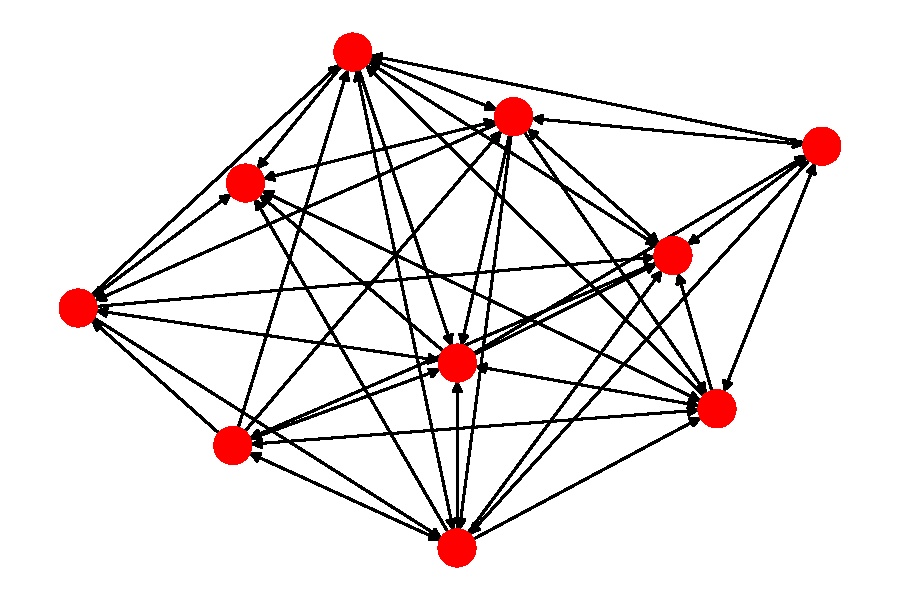
\includegraphics[width=.8\textwidth]{graph.pdf}
    \label{fig:image_of_graph}
\end{figure}

Mae'r algorithm `Page Rank' yn tybio bod defnyddwyr yn mynd i bori'r we ar hap
lle byddant yr un mor debygol o fynd o un wefan i unrhyw wefan arall y mae'r
wefan bresennol wedi'u cysylltu iddynt. Mae'r sg\^{o}r wrth ymyl pob gwefan yn
cyfateb \^{a}'r tebygolrwydd o fod ar y wefan honno:

\begin{minted}{python}
>>> nx.pagerank(G, alpha=1)
{0: 0.11988980099060496,
 1: 0.11337734639341283,
 2: 0.09229073511280955,
 3: 0.08488079369061019,
 4: 0.12554165518523688,
 5: 0.09448445809607922,
 6: 0.09608526108105925,
 7: 0.09314704994034195,
 8: 0.09384213164925923,
 9: 0.08646076786058658}
\end{minted}

\section{Defnyddio algebra llinol}

Byddwn yn normaleiddio \(A\) i greu matrics newydd \(M\) fel bod pob rhes yn
symio i un (fel bod pob rhes yn rhoi'r tebygolrwydd o fynd i'r wefan nesaf):

\begin{minted}{python}
>>> symiau_rhes = A.sum(axis=1)
>>> M = A / symiau_rhes[:, np.newaxis]
>>> np.round(M, 2)
array([[0.  , 0.12, 0.12, 0.  , 0.12, 0.12, 0.12, 0.12, 0.12, 0.12],
       [0.33, 0.  , 0.  , 0.33, 0.  , 0.  , 0.  , 0.  , 0.  , 0.33],
       [0.  , 0.17, 0.17, 0.  , 0.  , 0.17, 0.17, 0.17, 0.17, 0.  ],
       [0.17, 0.  , 0.17, 0.  , 0.17, 0.17, 0.  , 0.17, 0.17, 0.  ],
       [0.  , 0.14, 0.  , 0.14, 0.14, 0.14, 0.14, 0.14, 0.  , 0.14],
       [0.  , 0.17, 0.17, 0.17, 0.17, 0.  , 0.17, 0.  , 0.  , 0.17],
       [0.33, 0.  , 0.33, 0.  , 0.33, 0.  , 0.  , 0.  , 0.  , 0.  ],
       [0.2 , 0.2 , 0.  , 0.  , 0.  , 0.2 , 0.2 , 0.  , 0.2 , 0.  ],
       [0.  , 0.14, 0.  , 0.14, 0.14, 0.14, 0.14, 0.14, 0.14, 0.  ],
       [0.2 , 0.2 , 0.  , 0.  , 0.2 , 0.  , 0.  , 0.2 , 0.2 , 0.  ]])
\end{minted}

Gan ddefnyddio hwn, gallwn godi \(M\) i b\^{w}er mawr iawn i weld y
tebygolrwyddau rhediad hur yn dechrau ar unrhyw dudalen a rhoddir.

\begin{minted}{python}
>>> np.round(np.linalg.matrix_power(M, 2000000), 2)
array([[0.12, 0.11, 0.09, 0.08, 0.13, 0.09, 0.1 , 0.09, 0.09, 0.09],
       [0.12, 0.11, 0.09, 0.08, 0.13, 0.09, 0.1 , 0.09, 0.09, 0.09],
       [0.12, 0.11, 0.09, 0.08, 0.13, 0.09, 0.1 , 0.09, 0.09, 0.09],
       [0.12, 0.11, 0.09, 0.08, 0.13, 0.09, 0.1 , 0.09, 0.09, 0.09],
       [0.12, 0.11, 0.09, 0.08, 0.13, 0.09, 0.1 , 0.09, 0.09, 0.09],
       [0.12, 0.11, 0.09, 0.08, 0.13, 0.09, 0.1 , 0.09, 0.09, 0.09],
       [0.12, 0.11, 0.09, 0.08, 0.13, 0.09, 0.1 , 0.09, 0.09, 0.09],
       [0.12, 0.11, 0.09, 0.08, 0.13, 0.09, 0.1 , 0.09, 0.09, 0.09],
       [0.12, 0.11, 0.09, 0.08, 0.13, 0.09, 0.1 , 0.09, 0.09, 0.09],
       [0.12, 0.11, 0.09, 0.08, 0.13, 0.09, 0.1 , 0.09, 0.09, 0.09]])
\end{minted}

Gwelwn fod holl resi \(M ^ {2000000}\) yn hafal ac maent yn cyfateb \^{a}'r
gwerthoedd a chyfrifon trwy ddefnyddio `Page Rank' networkx.

Yn ddiddorol, gall cael y set o debygolrwyddau hyn trwy ganfod fector eigen de
\(M^{T}\):

\begin{minted}{python}
>>> gwerthoedd_e, fectorau_e = np.linalg.eig(M.T)
>>> np.real(np.round(fectorau_e[:,0] / sum(fectorau_e[:,0]), 2))
array([0.12, 0.11, 0.09, 0.08, 0.13, 0.09, 0.1 , 0.09, 0.09, 0.09])
\end{minted}

\section{Casgliad}

Roedd fersiwn cyntaf chwilotodd we Google yn seiliedig ar sylfeini algebra
llinol a theori graffiau. Roedd angen gwneud rhai newidiadau i ddeilio gyda'r
ffaith nid yw'r we trwy'r amser yn gysylltiedig yn gyfan gwbl, mae hyn yn
cyfateb \^{a}'r ddadl \texttt{alpha} yn y ffwythiant networkx uchod.

\bibliographystyle{plain}
\bibliography{bibliography.bib}


\end{document}
